\documentclass[a4paper,twoside,12pt,DIV=13,BCOR=5mm,numbers=noenddot,cleardoublepage=empty]{scrbook}
%======= Einbinden der benötigten Packete (= Zusatzfunktionen)
\usepackage[T1]{fontenc}                % für Fonts in westeuropäischer Codierung
\usepackage{lmodern}										% Latin Modern Paket verändert die verwendete Schriftart. Bessere Darstellung für pdf
\usepackage{textcomp}										% Provides extra symbols, e.g. arrows like \textrightarrow, various currencies (\texteuro,..
\usepackage[latin1]{inputenc}    				% german special characters
\usepackage[english,ngerman]{babel}     % hyphenation   usepackage[english,ngerman]{babel} f. deutsch
\usepackage{pdfpages}										% Einbinden von pdf-Files
\usepackage{pifont,textcomp,mathcomp}   % dingbad psfonts and text-compilant fonts (euro, TM, ...)
\usepackage{amsmath,amsopn,amsthm}      % AMS mathematics
\usepackage{amssymb}                    % zusätzliche Symbole 
\usepackage{xspace}											% avoids eaten spaces

%======= Eine Umgebung für Bilder und Tabellen			  	
%\usepackage[textfont={Small},labelfont={bf},margin=1cm,format=plain,font=singlespacing]{caption}   % hanging caption text [hang]
\usepackage[textfont={small},labelfont={bf},margin=1cm,format=plain,font=singlespacing]{caption}   % hanging caption text [hang]
\captionsetup*[figure]{name=Abb.}			 % Abbildungsunterschrift beginnt mit Abb.
\captionsetup*[table]{name=Tab.}


%======= Farben für Überschriften
\usepackage{color}
\definecolor{TUBlau}{rgb}{0,0.4,0.6}   % TU-blau RGB 0 102 153
\addtokomafont{sectioning}{\sffamily\bfseries\selectfont\color{TUBlau}}
\setkomafont{chapter}{\normalfont\huge\sffamily\bfseries\color{TUBlau}}
\addtokomafont{section}{\Large}
\addtokomafont{subsection}{\normalfont\Large\sffamily\bfseries\color{TUBlau}}
\addtokomafont{subsubsection}{\normalfont\large\sffamily\bfseries\color{TUBlau}}
\addtokomafont{paragraph}{\normalfont\large\sffamily\bfseries\color{TUBlau}}


%======= Kopf-/Fußzeilen
\pagestyle{plain} % nur Fußzeile



%======= Eine kompakte Umgebung für die Bilder
\newcommand{\bild}[4]{{
\begin{figure}[#2]
\begin{center}
\includegraphics[scale=#3]{pictures/#1}
\caption{#4}\label{fig:#1}
\end{center}
\end{figure}
}}


%======= Definitionen eigener Befehle
\newcommand{\degC}{\ensuremath{^{\circ}}C}        % Grad Celsius
\newcommand{\Gu}{\glqq{}}                         % Gänsefüßchen unten
\newcommand{\Go}{\grqq{}\xspace}    												% Gänsefüßchen oben











 
\usepackage{ucs} 	
\usepackage{float}		% File mit den ben�tigten Packeten, den Formatanweisungen und den Befehlsdefinitionen
\usepackage{graphicx}

\begin{document}


%===============================================================================
% Text
%===============================================================================

\cleardoublepage
\setcounter{tocdepth}{3}

\setcounter{page}{0}
\renewcommand{\thepage}{\roman{page}}
\tableofcontents \cleardoublepage

\setcounter{page}{1}
\renewcommand{\thepage}{\arabic{page}}
\setcounter{chapter}{0}


%===============================================================================

\newpage
\chapter{Zusammenfassung}
Die Zusammenfassung
\chapter{Ringkerntrafo}
\section{Aufnahme einer Hystereseschleife}

\section{Aufnahme der Permeabilit\"atskurve}
\subsection{Hintergrund}
Wird aus der Schaltung zur Aufnahme der Hystereseschleife der Integrator entfernt, steht die gemessene Spannung nicht mehr in Proportion 
zum Fluss durch die Spule, sondern zu seiner \"Anderungsrate. In diesem Fall kann das Entfernen des Integrators mit dem Ableiten der Funktion
gleichgesetzt werden. Betrachten wir das Verh\"altnis aus der \"Anderungsrate der Feldst\"arke und der \"Anderungsrate der Flussdichte sprechen wir von 
differenzieller Permeabilit\"at. Wird diese noch durch die Permeabilit\"at des Vakuums geteilt, erhalten wir die relative differenzielle Permeabilit\"at. Ziel ist es diese zu messen 
und auf plausibilit\"at zu pr\"ufen, sowie ihren Spitzenwert zu finden.
\subsection{Messergebnisse}
\begin{figure}
  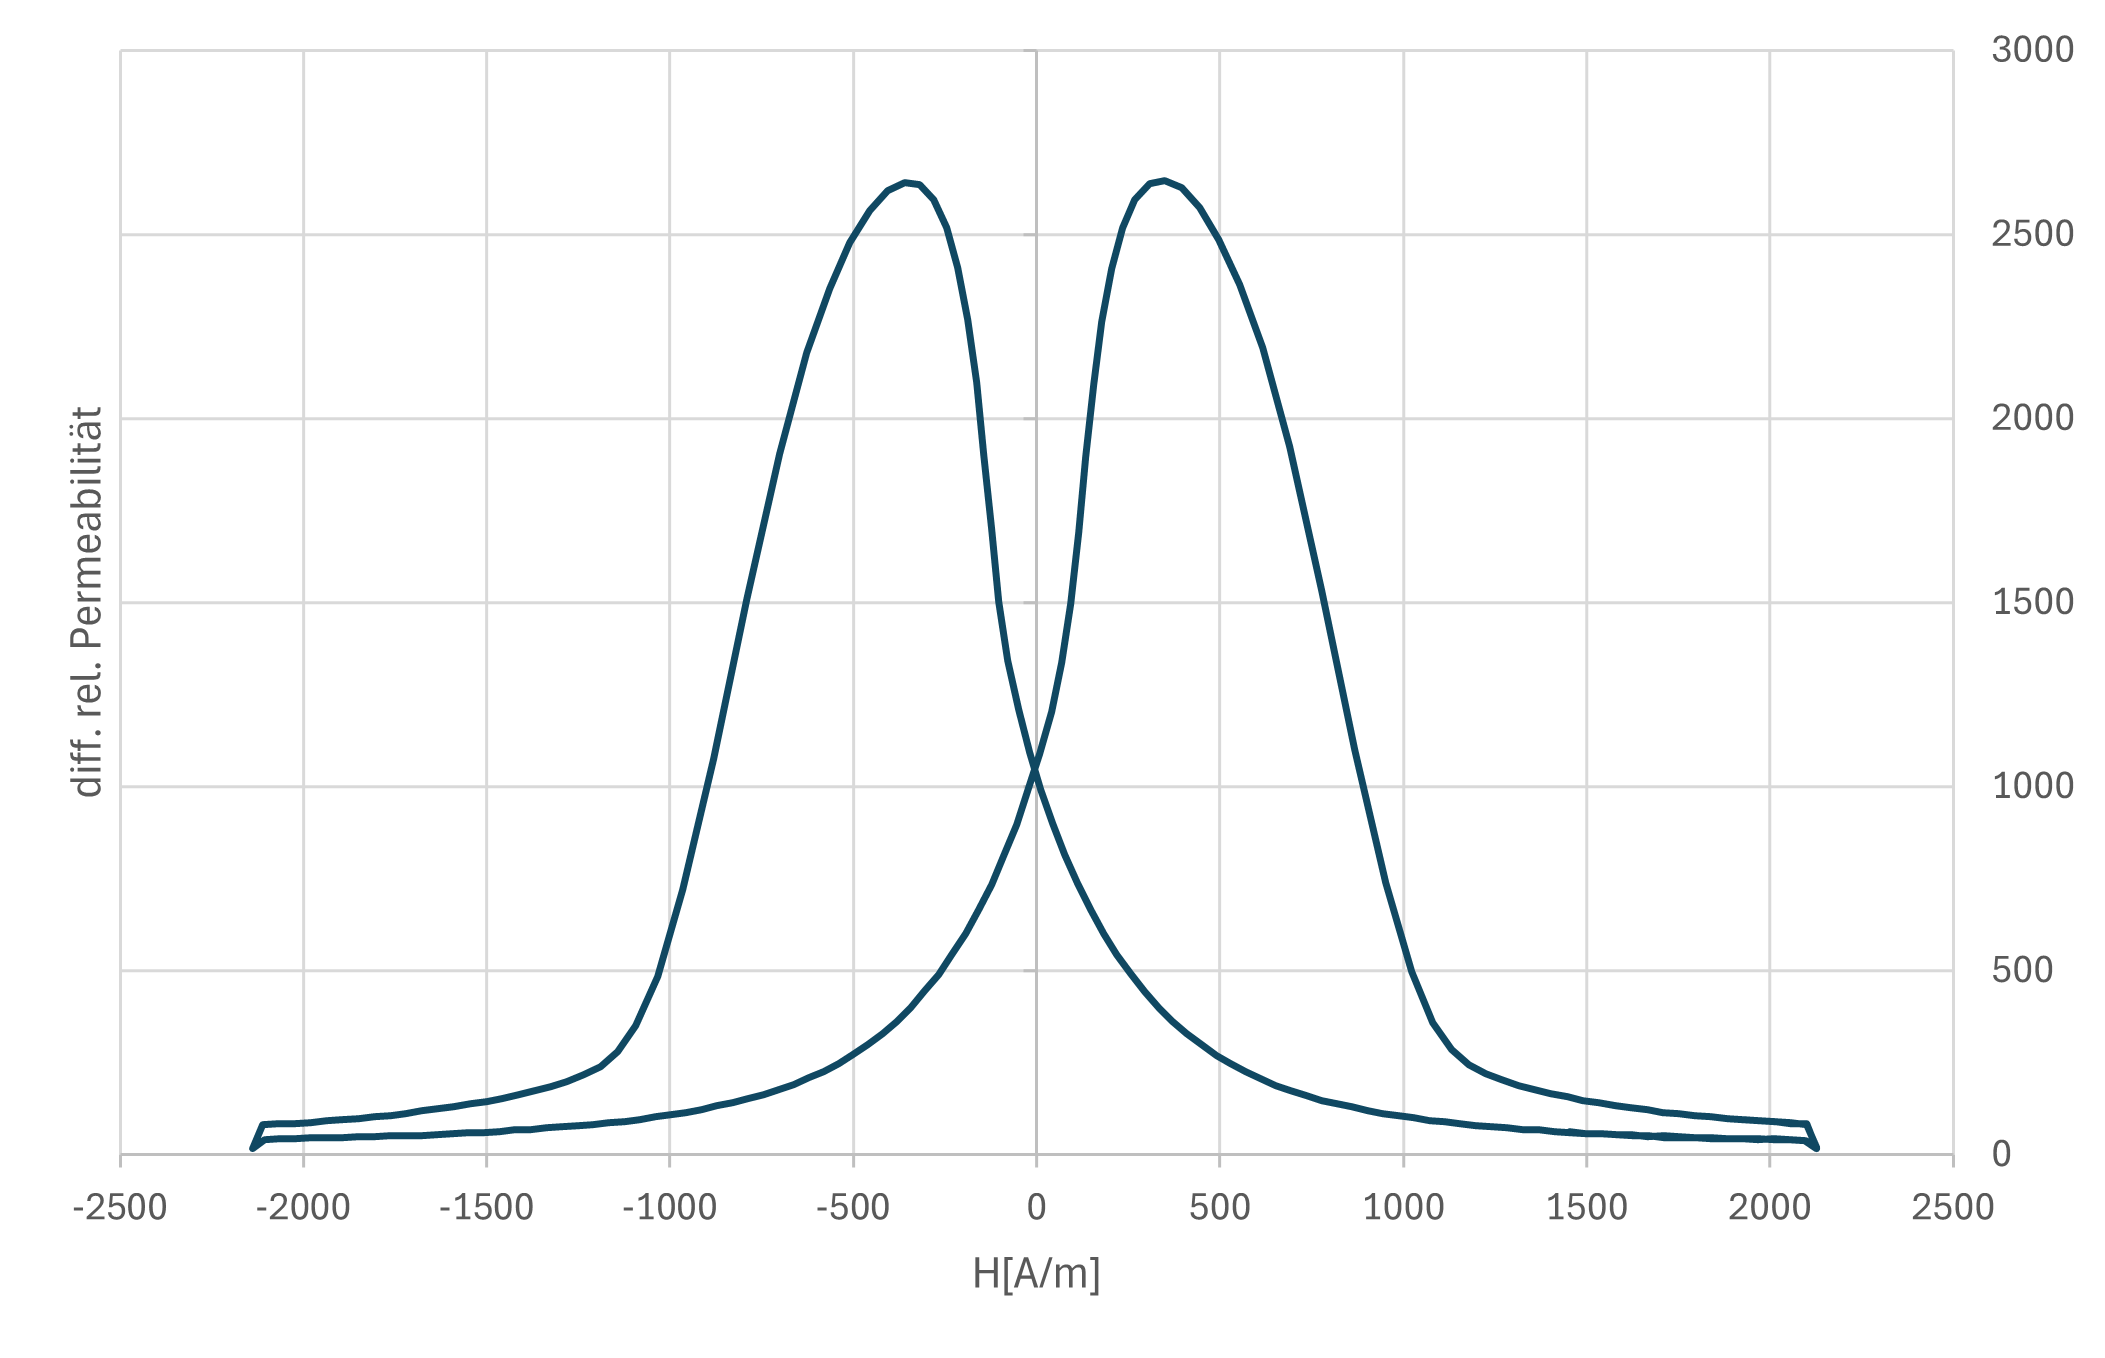
\includegraphics[width=\linewidth]{pictures/Permeabilitaet.png}
  \caption{Differenzielle relative Permeabilit\"at abh\"angig von der Feldst\"arke.}
  \label{fig:perm}
\end{figure}
Das Diagramm \ref{fig:perm} zeigt die gemessene differenzielle relative Permeabilit\"at abh\"angig von der Feldst\"arke. Ihr H\"ochstwert liegt bei etwa  2600. 
Vergleichen wir diesen Wert mit der g\"angigen relativen Permeabilit\"at f\"ur Eisen liegt der gemessene Wert in einem plausiblen Rahmen.

\section{Hysteresefamilie und Entmagnetisierung}
\label{Entmag}
\subsection{Setup}
Um die Neukurve (siehe \ref{Neukurve}) aufnehmen zu k\"ofnnen, braucht es einen unmagnetisierten Werkstoff. 
Der Ringkern wird dazu wiederholt, immer schw\"acher werdend, ummagnetisiert, wobei die Remanenz jedes mal kleiner wird.
Die dabei entstehende Zusammensetzung aus schw\"acher werdenden Hystereseschleifen wird als Hystesresefamilie bezeichnet. 
Um einen kontinuierlich schw\"acher werdenden Sinusstrom durch die Elektromagneten zu schicken wird das Signal des Funktionsgenerators 
mit der Spannung eines sich entladenden Kondendsators moduliert. Der Funktionsgenerator liefert unmoduliert eine Sinusspannung von 20Vpp  mit einer Periodendauer von zehn Sekunden.
Die RC Schaltung mit deren Spannung die des Funktionsgenerators moduliert wird besitzt eine Zeitkonstante von 60s. Die induzierte Spannung an der Messpule wird f\"ur diese Messung integriert. 
Die Widerstandswerte bleiben gleich.
\subsection{Messergebnisse}
\begin{figure}
  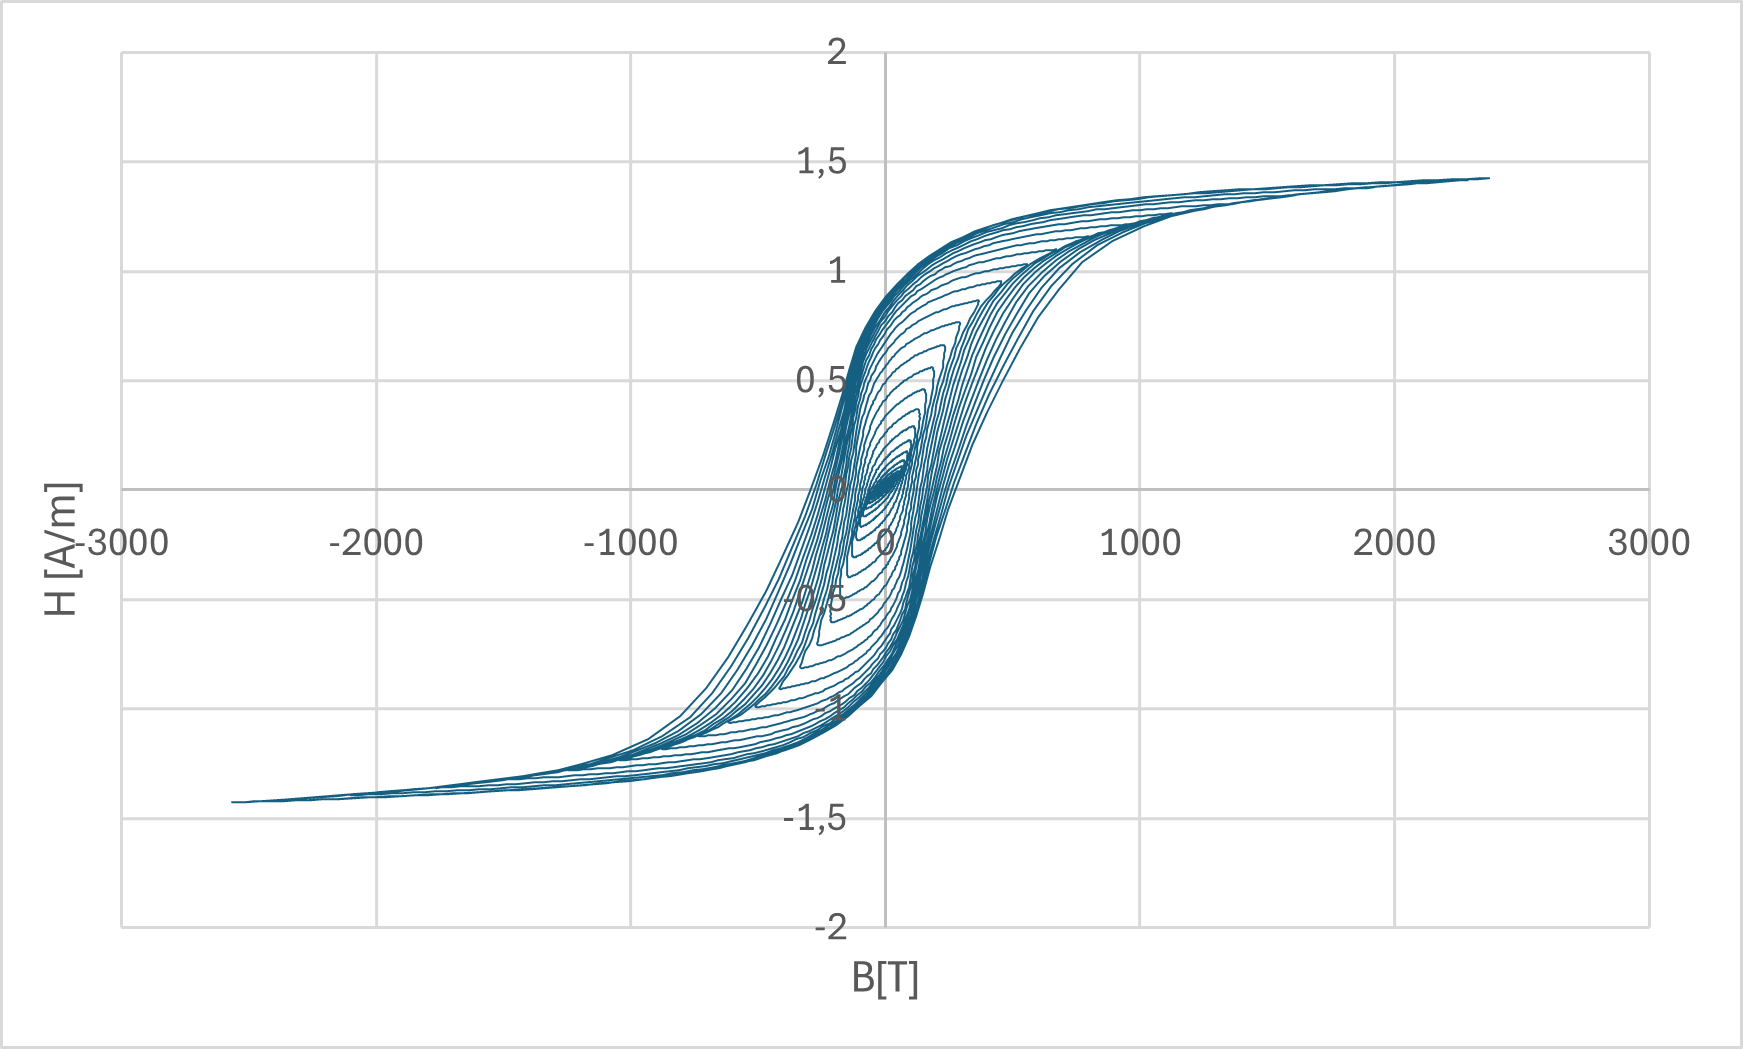
\includegraphics[width=\linewidth]{pictures/Hysteresefamilie.png}
  \caption{Hysteresefamilie, die die Entmagnetisierung des Ringkerns zeigt.}
  \label{fig:entmag}
\end{figure}
In dem Diagramm \ref{fig:entmag} kann sch\"on die Entmagnetisierung des Materials durch die immer kleiner werdenden Hystereseschleifen betrachtet werden.

\section{Die Neukurve}\label{Neukurve}
\subsection{Setup}
Ziel dieser Messung ist es eine Hystereseschleife inklusive einer Neukurve aufzunehmen. 
Dazu wird der gleiche Messaufbau wie beim einfachen Messen der Hystereseschleife verwendet. Anders ist in diesem Fall aber, dass der Kern des Trafos entmagnetisiert wurde (siehe \ref{Entmag}) und 
die Dreiecksspannung nur als zwei Zyklen Burst mit sechs Volt Spitze-Spitze angelegt wird.
\subsection{Messergebnisse}
\begin{figure}
  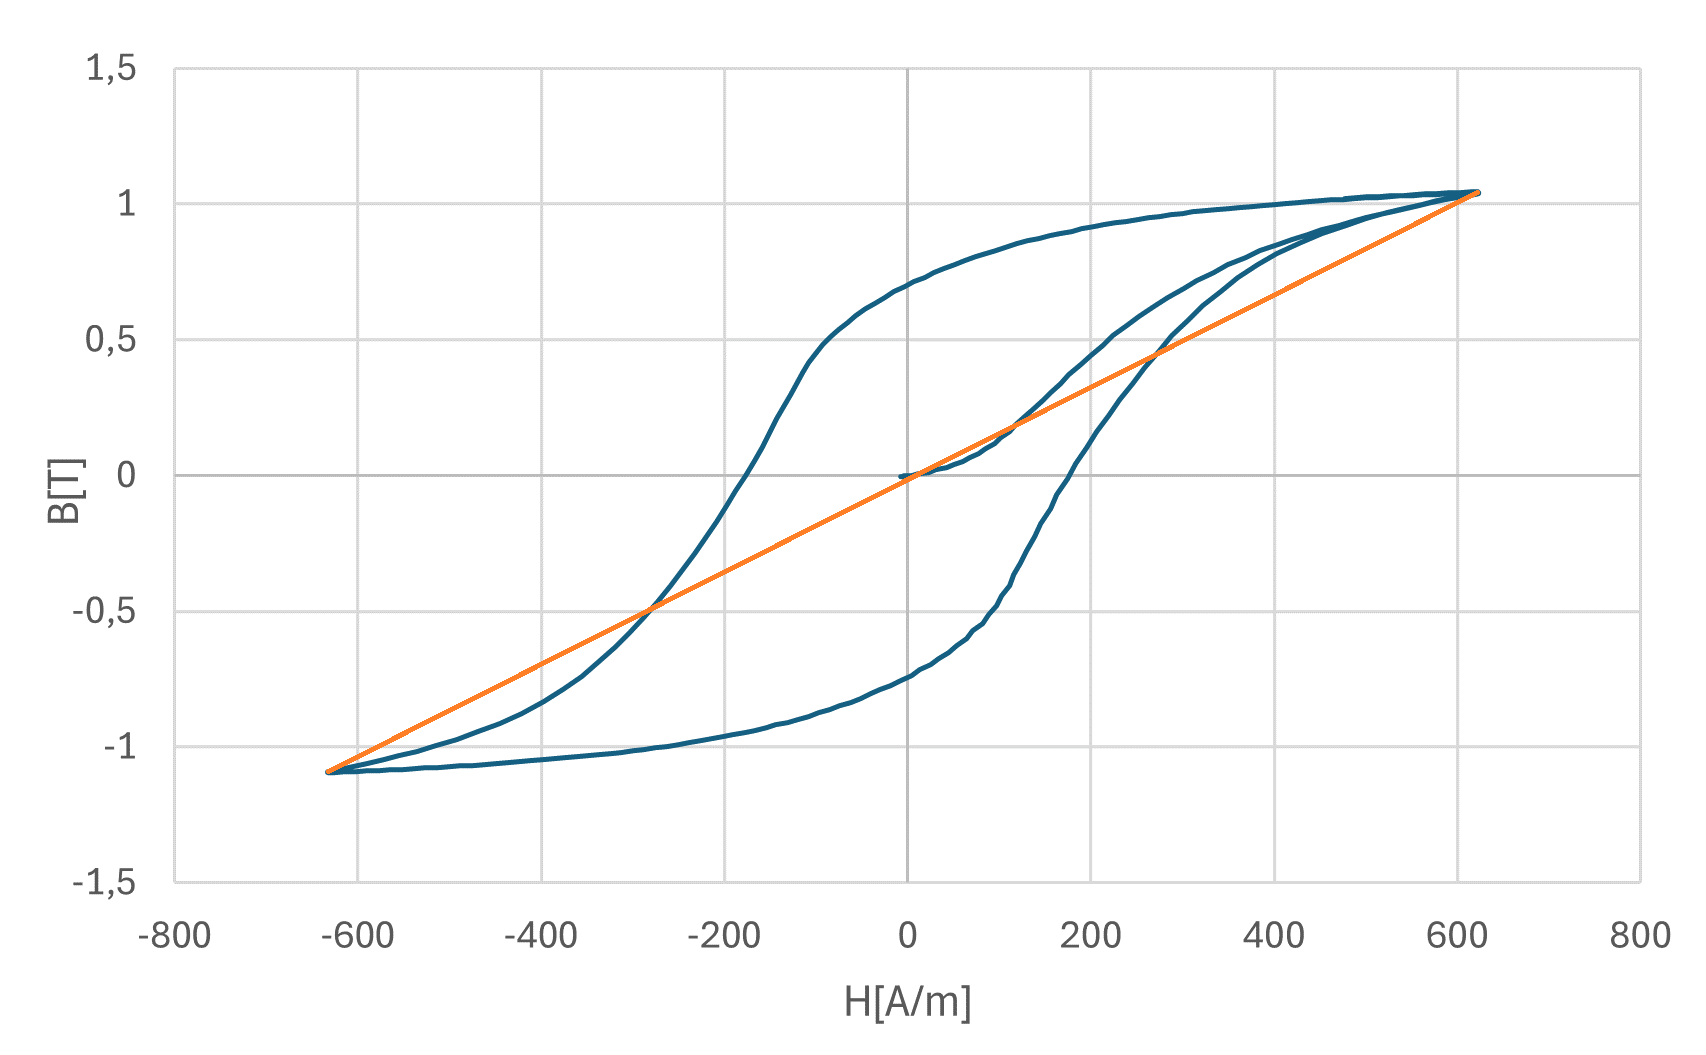
\includegraphics[width=\linewidth]{pictures/Neukurve.png}
  \caption{Hystereseschleife mit Neukurve, orange Gerade zur Symmetriepr\"ufung}
  \label{fig:neukurve}
\end{figure}
Im Diagramm \ref{fig:neukurve} sehen wir die bereits bekannte Hystereseschleife mit einer zus\"atzlichen Neukurve die das initale Magnetisieren des unmagnetisierten Stoffes darstellt.
 Der Integrator ist unter der Annahme, dass das Material vollst\"andig entmagnetisiert wurde zu Beginn der Messung zur\"uckgesetzt worden. Betrachten wir jetzt aber die Messwerte ist fest zu stellen, dass der Fluss nicht 
 in beiden Richtungen die gleiche Auslenkung besitzt. Zur besseren Visualisierung ist im Diagramm \ref{fig:neukurve} eine Linie zwischen den Spitzen der Schleife eingezeichnet. 
 Daraus ist zu erkennen, dass der Eisenkern zuvor nicht vollst\"andig entmagnetisiert wurde. 


 \chapter{\"ubungen am Elektromagneten}


\end{document}


